% !TEX root = ../gnss_interference_resistant_thesis.tex
\documentclass[main.tex]{subfiles}

\begin{document}

\subsection{Imtuvų fazės kalibravimas naudojant GNSS signalą}\label{sec:phase_clib_using_gnss}

Kaip aprašyta ankstesniuose skyriuose, naudojant HackRF SDR imtuvus, kiekvieno
matavimo pradžioje reikalingas fazinis imtuvų kalibravimas. Norint supaprastinti
matavimo metodiką, faziniam kalibravimui naudojamas priimamas GPS signalas.

Tam, kad būtų galima atlikti fazių nuokrypio įvertinimą, palydovas, naudojamas kalibravimui,
turi būti gerai matomas, bei jis turi būti dangaus skliauto viršuje.
Kai palydovas yra statmenai antenų masyvui, visos priimamos fazės visuose
imtuvuose turi būti lygios 0. Dėl šios priežasties, matavimus reikia
planuotis iš anksto, tuo laiku kai bent vienas palydovas yra
kuo aukščiau virš horizonto. Tinkamas palydovų išsidėstymas
pateiktas \ref{fig:gnss_sat_pos_calibartion}~pav.,
kalibravimui tinkamas palydovas yra PRN29.

\begin{figure}[ht]
    \begin{centering}
    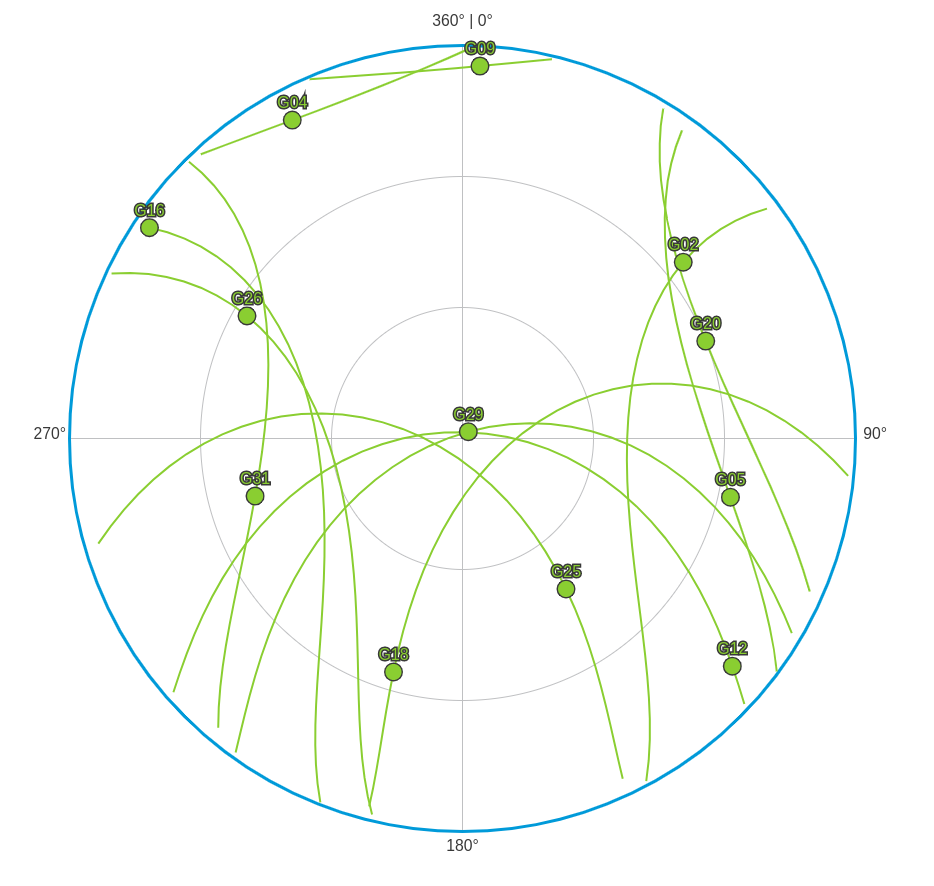
\includegraphics[scale=1.2]{drawings/gnss_sattelites_position}
    \par\end{centering}
    \protect\caption{\label{fig:gnss_sat_pos_calibartion}GPS palydovų pozicijos dangaus skliaute, adresu Saulėtekio al. 9, Vilnius, 2022-05-11 13:20.}
\end{figure}

Kalibravimas atliekamas lyginant vienos iš antenų fazę, su kitų trijų antenų fazėmis.
Atliekamas vidurkio skaičiavimas, gauta vertė atitinka fazės nuokrypį nuo tikrosios
fazės, ši vertė naudojama fazės poslinkiui visuose skaičiavimuose.

Jeigu palydovas nėra statmenas antenų masyvui, pritaikius spindulio formavimo
algoritmą, galime suskaičiuoti fazes kiekvienoje antenoje ir šis pokrypis
yra pridedamas prie nulinės fazės.

\subsection{GNSS signalo krypties nustatymas}\label{sec:gnss_doa_block}

Norint aptikti trikdžių šaltinius (pvz. signalo atspindžius), reikia žinoti
signalo priėmimo kryptį. Tai galima pasiekti pasinaudojus MUSIC krypties nustatymo
algoritmu (\ref{sec:music} skyrius), tačiau kadangi GPS signalo lygis yra
žemesnis už imtuvo triukšmus
ir visi GPS palydovai transliuoja tame pačiame dažnyje,
tiesiogiai imtuvo duomenims MUSIC taikyti negalime.

Krypties nustatymą galima įgyvendinti panaudojus GNSS signalo sekimo bloką,
aprašytą \ref{sec:tracking_block} skyriuje. GPS signalo sekimas yra vykdomas
vienoje iš antenų, pvz. $x_0[n]$. Tarpiniai sekimo rezultatai, nešlys ir
tikrojo signalo kopija $d_P[k]$, koreliuojami su
kitų antenų signalais, kaip pavaizduota \ref{fig:gnss_sdr_tracking_block_doa}
pav.

\begin{figure}[h]
    \begin{centering}
    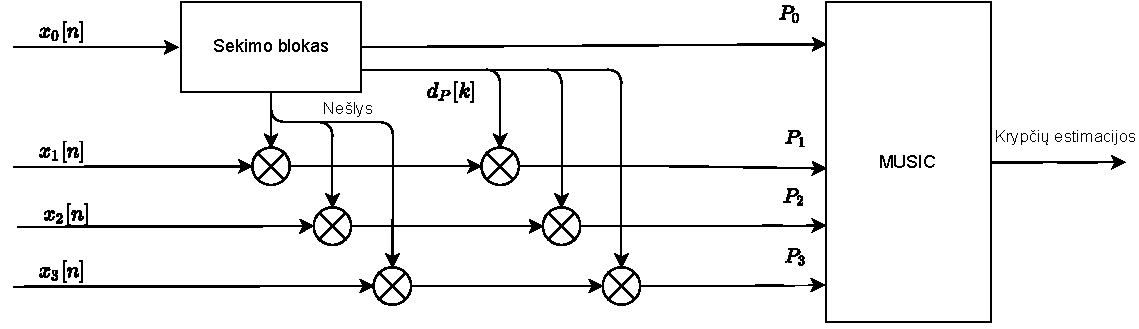
\includegraphics[scale=0.85]{drawings/tracking_diagram_doa}
    \par\end{centering}
    \protect\caption{\label{fig:gnss_sdr_tracking_block_doa}GNSS signalo krypties nustatymo diagrama.}
\end{figure}

Gautas koreliacijos rezultatas ($P_n$) yra kompleksinis skaičius, kurio
fazė parodo priimtų signalų fazes, todėl naudojantis
šiais duomenimis, galime nustatyti signalo priėmimo kryptį.
Koreliacijos rezultatai yra perduodami MUSIC algoritmui, kurio
įgyvendinimas atliktas panaudojus Python biblioteka "doatools.py" \cite{7738579}.

\ref{fig:gnss_sdr_tracking_block_doa}~pav. blokas yra vykdomas visuose
GNSS imtuvo kanaluose, todėl galime visų matomų palydovų signalų kryptis
nustatyti nepriklausomai. Gavus signalų kryptis ir žinant tikrąsias
palydovų padėtis galime pritaikyti spindulio formavimo algoritmą
arba pozicijos skaičiavimams nenaudoti palydovų, kurių signalas
yra priimamas netiesiogiai.

\end{document}
